\documentclass[useAMS,usenatbib,referee]{biom}

\usepackage{graphicx,epsfig,amssymb,amsmath,bm,bbm,natbib,xcolor}
\usepackage{Sweave}
\usepackage[colorinlistoftodos,linecolor=gray,backgroundcolor=white]{todonotes}   % to annotate text

% new command definitions
%\newtheorem{exercise}{Exercise}[chapter]
%\newtheorem{example}{Example}[chapter]
\newcommand{\ol}[1]{\overline{#1}}
\newcommand{\D}{\displaystyle}
\newcommand{\T}{\textstyle}
\newcommand{\s}{\scriptstyle}
\newcommand{\mc}[1]{\mathcal{#1}}
\newcommand{\bex}{\begin{exercise}}
\newcommand{\eex}{\end{exercise}}
\newcommand{\beg}{\begin{example}}
\newcommand{\eeg}{\end{example}}
\newcommand{\schist}[1]{\mbox{\tiny{#1}}}
\newcommand{\chist}[1]{\mbox{\scriptsize{#1}}}
\newcommand{\agemo}[1]{\mbox{$\underline{\omega}_{\/\downarrow #1}$}}
\newcommand{\ul}[1]{\mbox{$\underline{#1}$}}
\newcommand{\wh}[1]{\mbox{$\widehat{#1}$}}
\newcommand{\bv}{\begin{verbatim}}
\newcommand{\ev}{\end{verbatim}}
\newcommand{\bi}{\begin{itemize}}
\newcommand{\ei}{\end{itemize}}
\newcommand{\bfig}{\begin{figure}}
\newcommand{\efig}{\end{figure}}
\newcommand{\pref}[1]{\protect\ref{#1}}
\newcommand{\plab}[1]{\protect\label{#1}}
\newcommand{\be}{\begin{eqnarray}}
\newcommand{\bes}{\begin{eqnarray*}}
\newcommand{\ee}{\end{eqnarray}}
\newcommand{\ees}{\end{eqnarray*}}
\newcommand{\bo}[1]{\bf #1}
\newcommand{\bmt}[1]{\mbox{\boldmath $#1$}}
\newcommand{\tm}[1]{\mbox{\tiny{$#1$}}}
\newcommand{\vc}[2]{\mbox{$ \left[ \begin{array}{c} #1\\ \vdots \\ #2 
 \end{array} \right] $}}
\newcommand{\mt}[4]{\mbox{$ \left[ \begin{array}{c,c,c} #1 & \cdots & #2\\ 
 \vdots & \ddots & \vdots\\ #3 & \cdots & #4 \end{array} \right] $}}

\Sconcordance{concordance:paper.tex:paper.Rnw:%
1 4 1 1 0 81 1}

\bibliographystyle{chicago}


\title[2D or not 2D?]{Distance sampling: 2D or not 2D?}
\author{D.L. Borchers $^{*}$\email{dlb@st-andrews.ac.uk} \\
   Centre for Research into Ecological and Environmental Modelling, The Observatory \\
   Buchanan Gardens, University of St Andrews, Fife, KY16 9LZ, Scotland
   \and 
   M.J. Cox \\
   Australian Antarctic Division, Channel Highway Kingston TAS 7050,  Australia
   }

\begin{document}

\date{{\it Received XXXXX} 2014. {\it Revised XXXXX} 2014.  {\it
Accepted XXXXX} 2014.}

\pagerange{\pageref{firstpage}--\pageref{lastpage}}
\volume{??}
\pubyear{XXXX}
\artmonth{XXXXX}

\doi{10.1111/???}

\begin{abstract}
Distance sampling surveys occur in two spatial dimensions but conventional distance sampling (CDS) methods are one-dimensional, using only perpendicular (line transects) or radial (point transects) distances. These methods assume that animals are uniformly distributed in the vicinity of lines or points. But when animals move in response to observers before detection, or when lines or points are not located randomly, this assumption may fail. We show that two-dimensional models in which distances or times to first detections are used, allow simultaneous estimation of detection probability and this distribution. We also show that times to detection can provide evidence of failure of the CDS assumption that detection probability is 1 at distance zero, and in some circumstances may allow estimation of this probability. We formulate distance sampling models as survival models with an unknown number of right-censored subjects and distance as an individual random effect. We obtain a maximum likelihood estimator of line transect survey effective strip half-width and investigate its properties by simulation in situations where animals are nonuniformly distributed and their distribution is unknown. The estimator is found to perform well when detection probability at distance zero is 1 or close to 1. It allows estimates of density to be obtained from surveys in which there has been responsive movement prior to detection. We illustrate by estimating primate density from a line transect survey in which animals are known to avoid the transect line, and a shipboard survey of dolphins that are attracted to it.
\end{abstract}

\label{firstpage}

\begin{keywords}
$g(0)=1$, line transect, point transect, removal method, responsive movement, survival analysis
\end{keywords}

\maketitle

\section{Introduction\label{intro}}

There are two main distance sampling methods: line transects and point transects. On line transect surveys observers traverse lines and record at least the perpendicular distance from the line to detected individuals, while on point transect surveys observers survey from points and record at least the radial distances to detected individuals. Observers may also record the locations in the plane of detected individuals, and other covariates. See \cite{Marques+al:10} for a brief overview of distance sampling methods, and \cite{Buckland+al:01} for more detail.

Two key assumptions of distance sampling are (i) that individuals are distributed uniformly in space in the vicinity of the observers and (ii) that detection of individuals at distance zero is certain \citep{Buckland+al:01}. Assumption (ii) is referred to as the ``$g(0)=1$'' assumption in distance sampling literature, where $g(x)$ is the probability of detecting an individual that is at perpendicular distance $x$ in the case of line transects, and radial distance $x$ in the case of point transects. In this paper we use $p(x)$ rather than $g(x)$ for the detection function. Should either assumption be violated, abundance estimates may be biased. (Assumption (i) is 

Distance sampling surveys do not routinely record times to detection, although in the case of line transect surveys forward distances to detections are sometimes recorded and radial distance and angle from transect line are frequently recorded on shipboard surveys. Times to detection can be obtained from these if observer speed is known. Data on times to detection are easy to obtain on many distance sampling surveys, and we consider the utility of such data here. We show below that distance sampling methods that use times to detection are kinds of removal methods \citep[see][, Chapters 7 and 5, respectively, for an overview of removal methods]{Seber:82, Borchers+al:02}. And since removal methods do not require assumptions (i) and (ii), this suggests that unbiased abundance estimation from distance sampling surveys may be possible without these assumptions when data on times to detection are used. 

Historically, something akin to time to detection data were in fact used in many line transect survey models and we briefly review the reasons that their use was abandoned. But we start by looking at removal methods because these are closely related to distance sampling surveys with time to detection data, and the link with removal methods is useful for interpreting some aspects of the distance sampling models that we develop below.

\subsection{Removal models as survival models\label{sec:removal.surv}}

Removal methods involve repeated sampling of a population and removing animals from the population when they are detected or captured. (For brevity we refer to detection, capture and removal as ``detection'' henceforth.) In the simplest removal method, all animals are assumed to be equally detectable and sampling effort is assumed to be the same on each occasion. Variants include parameterising detection probability as a function of effort and inclusion of sex (for the ``change-in-ratio'' method) as an individual-level covariate. 

It is useful for our purposes to formulate a removal method with occasions $t=1,\ldots,T$ as a discrete time survival process with constant detection probability $p$ and an unknown number of right-censored individuals. In this case the ``survivor function'' (the probability of surviving) up to occasion $t-1$ is $S(t-1)=(1-p)^{t-1}$ and the probability of being detected at time (occasion) $t\leq T$ is $f(t)=S(t-1)p$ (i.e. $t$ has a geometric distribution). The likelihood for the abundance $N$ and and detection probability $p$, given that $n_t$ individuals were detected at time $t$ ($t=1,\ldots,T$) is multinomial, as follows:
\be
{\cal L}(N,p)
&=&\left(\frac{N!}{(N-n)!\prod_{t=1}^Tn_t!}\right) S(T)^{N-n}\prod_{t=1}^Tf(t)^{n_t} \nonumber \\
&=&\left(\frac{N!}{(N-n)!\prod_{t=1}^Tn_t!}\right) S(T)^{N-n}\prod_{i=1}^{n}S(t_i-1)p
\label{eq:simple.removal}
\ee

\noindent
where $n=\sum_t n_t$, $N-n$ is the unknown number of censored survival times. The focus of inference is the number of censored times. Although it is not usually formulated as a discrete survival model, the simple removal method likelihood \citep[see Equation 5.4 on page 76 of][for example]{Borchers+al:02} is identical to Eqn~(\ref{eq:simple.removal}). The essential equivalence of a constant-hazard survival model and the simple (constant detection probability) removal model is visually apparent by noting that the removal method plot of expected cumulative removals against time is the same as the plot of expected number of survivors against time, but with the y-axis inverted.

The link between removal methods and distance sampling methods becomes apparent when we consider the continuous-time analogue of the discrete-time removal model -- which we now do. We start by considering a survey of duration $T$ with fixed hazard per unit time of detection, $h$. In this case the survivor function at time $t$ is $S(t;h)=\exp\{-\int_0^th\;du\}=\exp\{-th\}$ and the probability density function (pdf) of the $n$ detection times, given detection, is $f(\bmt{t}|\bmt{t}<T)=\prod_{i=1}^n\frac{S(t_i;h)h}{1-S(T;h)}$, where $\bmt{t}<T$ indicates that $t_1,\ldots,t_{n}$ are all less than $T$. Note that $1-S(T;h)$ is the probability of detection by time $T$, which we denote $p$. The corresponding likelihood function (with unknown parameters $N$ and $h$) for the survey is ${\cal L}(N,h)=B\left(n;N,p\right)\prod_{i=1}^n\frac{S(t_i)h}{p}$, where $B\left(n;N,p\right)$ is a binomial distribution with index $N$ and ``success'' probability $p$, evaluated at $n$.

We now introduce a continuous individual random effect $x$ with pdf $\pi(x;{\bmt{\phi}})$ and parameter vector ${\bmt{\phi}}$, and we assume that individuals' $x$s are independent draws from this distribution. We allow the detection hazard to depend on both $x$ and time since the survey started, $t$. The detection hazard is now $h(t,x;{\bmt{\beta}})$, where ${\bmt{\beta}}$ is a vector of unknown parameters, the survivor function is $S(t,x;{\bmt{\beta}})$, and detection probability, conditional on $x$ is $p(x;{\bmt{\beta}})=1-S(T,x;{\bmt{\beta}})=1-\exp\{-\int_0^Th(u,x;{\bmt{\beta}})du\}$. The mean detection probability in the population is $p_\cdot({\bmt{\beta}},{\bmt{\phi}})=E_x[p(x;{\bmt{\beta}},{\bmt{\phi}})]=\int\pi(u;{\bmt{\phi}})p(u;{\bmt{\beta}})du$, where integration is over the survey region. The likelihood function can now be written as
\be
{\cal L}(D,{\bmt{\beta}})
&=&
B\left(n;N,p_\cdot({\bmt{\beta}},{\bmt{\phi}})\right)
\prod_{i=1}^n
\pi(x_i|\bmt{t}<T)f(\bmt{t}|x_i,\bmt{t}<T) \nonumber \\
&=&
B\left(n;N,p_\cdot({\bmt{\beta}},{\bmt{\phi}})\right)
\prod_{i=1}^n
\frac{\pi(x_i;{\bmt{\phi}})p(x_i;{\bmt{\beta}})}{\int\pi(u;{\bmt{\phi}})p(u;{\bmt{\beta}})du}
\frac{S(t_i,x_i;{\bmt{\beta}})h(t_i,x_i;{\bmt{\beta}})}{p(x_i;{\bmt{\beta}})} 
\label{eq:DSremoval1} \\
&=&
{N \choose n}[1-p_\cdot({\bmt{\beta}},{\bmt{\phi}})]^{N-n}\prod_i \pi(x_i;{\bmt{\phi}})S(t_i,x_i;{\bmt{\beta}})h(t_i,x_i;{\bmt{\beta}})
\label{eq:DSremoval2}
\ee

\noindent
The term $[1-p_\cdot({\bmt{\beta}},{\bmt{\phi}})]^{N-n}$ is for the unknown number ($N-n$) of censored survival times, which is the focus of inference.

\subsection{Distance sampling models as survival models\label{sec:DS.surv}}

Although they are traditionally treated as instantaneous surveys, distance sampling surveys seldom really are. An individual at distance $x$ is in view for some period (of length $T$ say), and at times $0\leq t\leq T$ it has some hazard $h(t,x;{\bmt{\beta}})$ of being detected. And although individuals detected on distance sampling surveys are not physically removed, they are effectively removed if the usual distance sampling protocol of recording only the locations of individuals when first detected, is used. In this case, one can consider a distance sampling survey to be a removal survey of the sort described immediately above, and hence also as a kind of survival model survey. 

Indeed, the conventional distance sampling full likelihood is identical to Equation~(\ref{eq:DSremoval1}) with the random effect $x$ being perpendicular distance, except that in distance sampling (a) the random effect distribution $\pi(x_i;{\bmt{\phi}})$ is treated as known, and (b) the term with detection times ($f(\bmt{t}|x_i,\bmt{t}<T)=S(t_i,x_i;{\bmt{\beta}})h(t_i,x_i;{\bmt{\beta}})/p(x_i;{\bmt{\beta}})$) is omitted - see \cite{Buckland+al:04}, Equation~(2.33) or \cite{Borchers+al:02}, Equation~(7.10). This raises the question of why $f(\bmt{t}|x_i,\bmt{t}<T)$ is omitted from distance sampling likelihoods -- something that reduces the data from two dimensions ($x$ and $t$) to one dimension ($x$). In the case of line transect surveys, the answer can be found in a landmark paper by \cite{Hayes+Buckland:83}.

\subsection{Line transect surveys}

\cite{Hayes+Buckland:83} considered a number of line transect models that included forward distances. (Using forward distance, $y$, is equivalent to using times to detection if observers move at constant speed, $v$, since $y=y_{max}-vt$, where $y_{max}$ is some large forward distance used as a reference point). These models were formulated in terms of perpendicular and radial distance rather than perpendicular and forward distance, but it is straightforward to switch between the two. They key point is that they are two-dimensional (2D) line transect models and the key question here is why 2D models were abandoned. 

\citet{Hayes+Buckland:83} considered the 2D models of \cite{Hayne:49}, \cite{Eberhardt:78}, \cite{Burnham+Anderson:76} and \cite{Burnham:79}. These are all based on rather restrictive assumptions about the detection process and in their examination of these models, \citet[][p 33]{Hayes+Buckland:83} conclude that ``none of the models appears to be founded upon realistic assumptions.'' They went on to develop a ``hazard rate'' model for the detection process. Although they did not call it this, their model is a survival model just like that developed in Section~\ref{sec:removal.surv} above, with a detection hazard that depends on forward and perpendicular distance.

The model of \cite{Hayes+Buckland:83} used a hazard function, $k(r,x)$, formulated it in terms of radial distance $r$ and perpendicular distance $x$, rather than time and perpendicular distance as in Section \ref{sec:removal.surv}, but it is straightforward to switch between the two formulations. Their key conclusion with regard to density estimators ($\hat{D}$) from 2D hazard models was (p39) ``We do not believe that the estimator $\hat{D}$ will be robust to the form arbitrarily chosen for $k(r,x)$ when observed radial distances are used for estimation.''\footnote{\cite{Hayes+Buckland:83} use $y$ for perpendicular distance; we use $x$. We have changed ``$k(r,y)$'' to ``$k(r,x)$'' in this quotation for consistency with our notation.} They also went on to develop a new form of perpendicular distance detection function (the now well-known ``hazard rate'' form) based on their survival model, and showed that this form is obtained from a variety of forms for $k(r,x)$. 

The weakness of the 2D models that \cite{Hayes+Buckland:83} looked at was that they were ``arbitrary'' and ``founded on unrealistic assumptions''. But other 2D distance sampling models had been used successfully before 1983 \citep[][for example]{Schweder:74} and have been used successfully since. Examples include \citep{Schweder:90}, \cite{Schweder+al:96}, \cite{Schweder+al:97}, \cite{Schweder+al:99}, \cite{Skaug+Schweder:99}, \cite{Okamura:03}, \cite{Skaug+al:04}, \cite{Okamura+al:03}, \cite{Okamura+al:06}, \cite{Okamura+al:12}, \cite{Borchers+al:13}, \cite{Langrock+al:13} and  \cite{Borchers+Langrock:ip}. These papers used a variety of more flexible hazard function forms than the models considered by \cite{Hayes+Buckland:83}, including models that allow $p(0)<1$. However, all of them concern individuals that become available and unavailable for detection stochastically while within detection range, and we are not aware of any line transect models other than those considered by \cite{Hayes+Buckland:83} that use 2D detection models without also modelling stochastic individual availability. We develop such models here, using the hazard models proposed by \cite{Hayes+Buckland:83} and two of the hazard models proposed by the authors listed above. 

\subsection{Point transect surveys}

On line transect surveys, time to detection and forward distance are interchangeable so that once one is recorded the other contains no new information, but this is not the case on point transect surveys (because observers do not move), and hence time to detection may add new information on detection probability beyond that provided by angle and distance. To our knowledge, no models using time to detection have been proposed for point transect surveys to date, although 2D models that use angles in addition to the conventionally recorded radial distances to detections have been developed by \cite{Marques+al:10a}, \cite{Cox+al:11} and \cite{Arranz+al:14} to deal with non-uniform distribution of individuals. 

However, although they do not say so explicitly, these methods rely on the detection function gradient and density gradient not being coincident in order to separate change in detection probability from change in density. If the gradients coincide, the use of data on angles in addition to distances does not allow change in density to be separated from change in detectability. To deal with this limitation, \cite{Marques+al:10a} and \cite{Arranz+al:14} assumed that detection probability does not depend on angle, but density might, while \cite{Cox+al:11} obtained independent information on the rate of change of detection probability with angle. Because time to detection data are survival data, and detection probability can be estimated from survival data alone, the addition of time to detection data does in principle allow change in density to be separated from change in detectability.


\subsection{Detection probability at distance zero}

One can enforce a requirement that $p(0)=1$ by choosing an appropriate hazard function form - as did \cite{Hayes+Buckland:83}, for example. Or one can use a hazard rate form that does not require the $p(0)=1$ assumption, as did \cite{Langrock+al:13}, for example. 

Thinking of distance sampling data as removal data, one would expect that it is possible to estimate abundance without assuming that $p(0)=1$ - since no such assumption is required for estimation from removal method data. On the other hand, the simple (constant $p$) removal method performs poorly unless a relatively high proportion of the population is detected \citep[see][Table 7.3, for example]{Seber:82}, i.e., unless $S(T)$ is close to 1. So one might expect poor performance from 2D distance sampling estimators unless $p(0)=p(x=0;{\bmt{\beta}})=1-S(t,x=0;{\bmt{\beta}})$ is close to 1. We consider this further below.



\section{Distance sampling likelihood\label{sec:DSlikelihood}}
We focus on estimation of animal density within the covered region - the part of the survey region within some distance $w$ of the lines that observers traverse or the points at which they are located. We refer to the lines or points collectively as ``samplers''. If samplers were located along some geographic feature such as a path, then density within the covered region may not be representative of density beyond it and conventional (design-based) estimators of density in the survey region as a whole may yield biased estimates. The same is true if animals moved in response to the observers' presence, whether or not samplers were placed randomly. If the effect of the sampler location on animal distribution has disappeared by distance $w$ from the sampler, then it is possible to use the estimated density at distance $w$ as representative of density in the survey region as a whole. See \cite{Marques+al:10} for some discussion of this issue in the context of point transect methods. Here we focus on inference within the covered region.

\subsection{A survival model likelihood for distance sampling}
In this section we obtain a likelihood that is slightly more general than that in  Equation~(\ref{eq:DSremoval2}) in that it incorporates vector $\bmt{x}$ comprising Cartesian coordinates in the plane, rather than scalar $x$. We also assume Poisson rather than binomial form for the pmf of $n$.

We assume that animals occur independently in the plane according to a nonhomogeneous Poisson process (NHPP) with intensity $D({\bmt{x}};{\bmt{\phi}})$ at Cartesian coordinates ${\bmt{x}}=(x,l)$, where ${\bmt{\phi}}$ is a vector of unknown parameters. For convenience we orient the coordinates for line transect surveys such that $x$ is distance perpendicular to the line and $l$ distance along the line from the start of the line, while for point transect surveys we locate the observer at ${\bmt{x}}=(0,0)$. We further assume that animals are stationary for the duration of the survey. Each animal has its own time frame of reference, with 0 corresponding to a time before individuals are detectable and individuals being being at risk of detection from 0 to $T$. For $0\leq t \leq T$ the hazard of detecting an animal at ${\bmt{x}}$ is a function $h({\bmt{x}},t;{\bmt{\beta}})$, where ${\bmt{\beta}}$ is a vector of unknown parameters. The probability of detection is the complement of the ``survivor'' function: $p({\bmt{x}};{\bmt{\beta}})=1-S(T,{\bmt{x}};{\bmt{\beta}})$, with $S(T,{\bmt{x}};{\bmt{\beta}})=\exp\{-\int_0^T h({\bmt{x}},t;{\bmt{\beta}})dt\}$ being the survivor function. 

The survey data are the $n$ locations of detected animals in space and (animal-specific) time in view: ${\bmt{x}}=({\bmt{x}}_1,\ldots,{\bmt{x}}_{n})$ and ${\bf t}=(t_1,\ldots,t_{n})$.  We construct a likelihood by obtaining expressions for the distribution of $n$, the distribution of ${\bmt{x}}$ given $n$ ($f_{x|n}$), and the distribution of ${\bf t}$ given ${\bmt{x}}$ ($f_{t|x}$). These are
\begin{eqnarray}
P(n;{\bmt{\phi}},{\bmt{\beta}})&=&\frac{\lambda({\bmt{\phi}},{\bmt{\beta}})^ne^{- \lambda({\bmt{\phi}},{\bmt{\beta}})}}{n!}
\end{eqnarray}
\noindent
where $\lambda({\bmt{\phi}},{\bmt{\beta}})=\int\limits_{R^2} D({\bmt{x}};{\bmt{\phi}})p({\bmt{x}};{\bmt{\beta}})d {\bmt{x}}$ and integration is over the plane within distance $w$ of samplers, 
\begin{eqnarray}
f_{x|n}({\bmt{x}}|n)=\prod^{n}_{i=1} \frac{D({\bmt{x}}_i;{\bmt{\phi}})p({\bmt{x}}_i;{\bmt{\beta}})}{\lambda({\bmt{\phi}},{\bmt{\beta}})}
\end{eqnarray}
\noindent
and, using Bayes Theorem with a standard result from survival analysis,
\begin{eqnarray}
f_{t|x}({\bf t}|{\bmt{x}})=\prod^{n}_{i=1}\frac{S(t_i,{\bmt{x}}_i;{\bmt{\beta}})h({\bmt{x}}_i,t_i;{\bmt{\beta}})}{p({\bmt{x}}_i;{\bmt{\beta}})}.
\end{eqnarray}
\noindent
The product of the above three distributions gives our likelihood function:
\begin{eqnarray}
\mathcal{L}({\bmt{\phi}},{\bmt{\beta}})
&=&P(n;{\bmt{\phi}},{\bmt{\beta}})f_{x|n}({\bmt{x}}|n)f_{t|x}({\bf t}|{\bmt{x}}) 
\label{eq:full.lik} \\
&\propto& e^{-\lambda({\bmt{\phi}},{\bmt{\beta}})}\prod^{n}_{i=1}D({\bmt{x}}_i;{\bmt{\phi}})S(t_i,{\bmt{x}}_i;{\bmt{\beta}})h({\bmt{x}}_i,t_i;{\bmt{\beta}}).
\end{eqnarray}

Density is estimated by maximising this likelihood with respect to ${\bmt{\phi}}$ and ${\bmt{\beta}}$ and evaluating $D({\bmt{x}};\hat{\bmt{\phi}})$, where $\hat{\bmt{\phi}}$ is the value at which the likelihood is a maximum. Confidence intervals can be obtained using the inverse of the Hessian that is obtained from numerical maximisation of the the likelihood. 

Line transect and point transect surveys involve slightly different special cases of the above general likelihood function. We consider these in turn below.

\subsection{Point transect likelihood}
With stationary animals and stationary observer, we assume that the detection hazard is the same for all $t$ in the survey at any given location ${\bmt{x}}$ and hence write it as $h({\bmt{x}};{\bmt{\beta}})$. The the survivor function to time $t$ remains $S(t,{\bmt{x}};{\bmt{\beta}})$. The point transect version of the likelihood can therefore be written as follows (without dependence of $h(\;)$ on $t$):
\begin{eqnarray}
\mathcal{L}_{PT}({\bmt{\phi}},{\bmt{\beta}})\propto e^{-\lambda({\bmt{\phi}},{\bmt{\beta}})}\prod^{n}_{i=1}D({\bmt{x}}_i;{\bmt{\phi}})S(t_i,{\bmt{x}}_i;{\bmt{\beta}})h({\bmt{x}}_i;{\bmt{\beta}}).
\end{eqnarray}


\subsection{Line transect likelihood}
As with conventional line transect models, we start by assuming that that the probability of detecting an animal at perpendicular distance $x$ from the line does not depend its distance $l$ along the line. This implies that the detection hazard function depends on $x$ and time in view ($t$), but not on $l$, so that it can be written as $h(x,t;{\bmt{\beta}})$ and the survivor function can be written as $S(t,x;{\bmt{\beta}})$. (For the hazard not to depend on $l$, the ``end effect'' of animals near the start of a transect line being in view for less time than animals further down the line, must be negligible.) 
With $h(x,t;{\bmt{\beta}})$ and $S(t,x;{\bmt{\beta}})$ not depending on $l$, the likelihood can be integrated over $l$ without loss if one is not interested in the density with respect to $y$, to yield
\begin{eqnarray}
\mathcal{L}_{LT}({\bmt{\phi}},{\bmt{\beta}})\propto e^{-\lambda({\bmt{\phi}},{\bmt{\beta}})}\prod^{n}_{i=1}D_x(x_i;{\bmt{\phi}})S(t_i{\bmt{x}}_i;{\bmt{\beta}})h(x_i,t_i;{\bmt{\beta}}).
\label{eq:LTlik}
\end{eqnarray}
\noindent
where $D_x(x_i;{\bmt{\phi}})=\int D({\bmt{x}}_i;{\bmt{\phi}})dl$ and integration is over the length of the transect line.

\subsubsection{Conditional likelihood}

Inference in distance sampling is conventionally based on the conditional likelihood, given detection of $n$ objects, rather than the unconditional likelihood given above (which includes a probability model for $n$). This is to avoid having to model the distribution of objects outside of searched strips or circles \citep{Borchers+Burnham:04}. The conditional likelihood is
\begin{eqnarray}
\mathcal{L}_{cond}({\bmt{\phi}},{\bmt{\beta}})
&=&f_{x|n}({\bmt{x}}|n)f_{t|x}({\bf t}|{\bmt{x}}) 
\nonumber \\
&=&
\left\{\prod^{n}_{i=1} \frac{D({\bmt{x}}_i;{\bmt{\phi}})p({\bmt{x}}_i;{\bmt{\beta}})}{\lambda({\bmt{\phi}},{\bmt{\beta}})}\right\}
\left\{\prod^{n}_{i=1}\frac{S(t_i,{\bmt{x}}_i;{\bmt{\beta}})h({\bmt{x}}_i,t_i;{\bmt{\beta}})}{p({\bmt{x}}_i;{\bmt{\beta}})}\right\}
\label{eq:cond.lik}.
\end{eqnarray}

Here $f_{x|n}({\bmt{x}}|n)$ corresponds to the CDS conditional likelihood, but with a more general form for $D({\bmt{x}}_i;{\bmt{\phi}})$ than is conventionally used. With CDS, uniform object density within $w$ of the observer is assumed, so that $D({\bmt{x}}_i;{\bmt{\phi}})=C$ for some constant $C$, and $C$ cancels in $f_{x|n}({\bmt{x}}|n)$. If for line transects, we integrate out distance along the line, $l$, assuming that $p({\bmt{x}}_i;{\bmt{\beta}})$ does not depend on $l$, we get $\prod_i p(x_i;\boldsymbol{\beta})/\int p(x;\boldsymbol{\beta})dx$, which is the CDS conditional likelihood for line transects \citep[see][]{Buckland+al:01}. Similarly, assuming that $p({\bmt{x}}_i;{\bmt{\beta}})$ depends only on radial distance ($r$) for point transects and, changing variable in $f_{x|n}({\bmt{x}}|n)$ from Cartesian coordinates $(x,l)$ to polar coordinates $(r,\theta)$, and integrating out the angle to object ($\theta$), we get the CDS point transect conditional likelihood $\prod_i r_ip(r_i;\boldsymbol{\beta})/\int rp(r;\boldsymbol{\beta})dr$. CDS likelihoods do not use times to detection and do not involve the component $f_{t|x}({\bf t}|{\bmt{x}})$. We do include times to detection and $f_{t|x}({\bf t}|{\bmt{x}})$.


\subsection{CDF and PDF of detection times}

The shape of the probability denstiy function (PDF) of detection time $t$ at distance zero, for $t\leq T$, turns out to be somewhat informative about $p(0)$. It is 
\begin{eqnarray}
f_{t|x}(t|x;\boldsymbol{\beta}))&=&\frac{S(t,x;\boldsymbol{\beta})h(x,t;{\bmt{\beta}})}{1-S(T,x;\boldsymbol{\beta})}
\end{eqnarray}
evaluated at $x=0$. Now if $p(0)=1$ then $f_{t|x}(T|x=0;\boldsymbol{\beta}))$ must be equal to zero, as in this case no animals survive detection beyond $T$ (i.e. at forward distances $y<0$), and as a result there will be no detections at, or very close to $(x=0,y=0)$). This in turn means that $f_{t|x}(t|x;\boldsymbol{\beta}))$ must have a mode at $t<T$ ($y>0$). When it does not have such a mode, this implies that $p(0)$ is less than 1. 

The cumulative distribution function (CDF) of $t$ is the scaled probability that an object survives detection up to time $t$: $F_{t|x}(t,x;\boldsymbol{\beta})=S(t,x;\boldsymbol{\beta})/\int_0^T S(t,x;\boldsymbol{\beta})dt$. This is analogous to the removal method cumulative distribution function and as with removal methods, when $F_{t|x}(t=T,x;\boldsymbol{\beta})$ is not close to 1 (i.e. when, by the end of the period in which animals are at risk of removal/detection, not a large fraction of the available population has been removed/detected), estimation of the available population size, and hence proportion of the population that has been removed/detected (and specifically $p(0)=F_{t|x}(t=T,x=0;\boldsymbol{\beta})$ in the present context), can not be done reliably.

The mean pdf of $t$, given detection, is useful for visually assessing goodness of fit in the $t$ dimension. For line transects this is 
\begin{eqnarray}
E_x[f_{t|x}(t|x;\boldsymbol{\beta})]&=&\int_x^w f_{t|x}(t|x;\boldsymbol{\beta}))\pi(x;\boldsymbol{\phi})dx,
\end{eqnarray}
\noindent
where $\pi(x;\boldsymbol{\phi})=\frac{D_x(x;{\bmt{\phi}})}{\int D(x
;{\bmt{\phi}})dx}$ is the pdf of $x$ in the population (detected and undetected). 


\section{Detection hazards and perpendicular distance distributions}

Although our models are formulated above in terms of detection times, when observers move at constant speed it is convenient to work in terms of forward detection distances ($y$) rather than times, which we do henceforth. We use one of the hazard forms (model $h_{HB}$ below) proposed by \cite{Hayes+Buckland:83} as well as the exponential power and inverse power hazard models that were used by \cite{Langrock+al:13} ($h_{EP}$ and $h_{IP}$). We also generalise $h_{HB}$ to allow $p(0)<1$ (hazard $h_{HB1}$) and the latter two  to allow separate scale parameters for $x$ and $y$ (models $h_{EP1}$ and $h_{IP1}$). The models are as follows ($\beta_j>0$ for all $j$):
\begin{eqnarray}
h_{HB}(\boldsymbol{x};\boldsymbol{\beta})&=&\beta_1 (x^2+y^2)^{-(\beta_2+2)/2} \nonumber \\
%h_{HB2}(x;\boldsymbol{\beta})&=&\beta_0 y(x^2+y^2)^{-(\beta_1+3)/2}\;\;\;\;\;\;\;\;\;\;(\beta_1,\beta_2>0) \nonumber \\
h_{EP}(\boldsymbol{x};\boldsymbol{\beta})&=&\beta_1\exp\left\{\left(\frac{x}{\beta_2}\right)^{\beta_3}+\left(\frac{y}{\beta_2}\right)^{\beta_3}\right\} \nonumber \\
h_{IP}(\boldsymbol{x};\boldsymbol{\beta})&=&\beta_1\left\{1+\left(\frac{x}{\beta_2}\right)^2+\left(\frac{y}{\beta_2}\right)^2\right\}^{-(\beta_3+1)/2} \nonumber \\
h_{HB2}(\boldsymbol{x};\boldsymbol{\beta})&=&\beta_1 (x^2+(y+\beta_3)^2)^{-(\beta_2+2)/2} \nonumber \\
h_{EP2}(\boldsymbol{x};\boldsymbol{\beta})&=&\beta_1\exp\left\{\left(\frac{x}{\beta_2}\right)^{\beta_3}+\left(\frac{y}{\beta_4}\right)^{\beta_3}\right\} \nonumber \\
h_{IP2}(\boldsymbol{x};\boldsymbol{\beta})&=&\beta_1\left\{1+\left(\frac{x}{\beta_2}\right)^2+\left(\frac{y}{\beta_4}\right)^2\right\}^{-(\beta_3+1)/2} \nonumber
\end{eqnarray}
The hazard $h_{HB}$ has $p(0)=1$, whereas the other hazards allow $p(0)<1$. We use slightly different forms for $h_{EP}$ and $h_{IP}$ than do \cite{Langrock+al:13}, in that we allow $\beta_1$ to be greater than 1 (because our hazard functions are rates, not probabilities). 

As is done with CDS methods, we use the absolute value of perpendicular distance so that $x\geq 0$, and we right-truncate $x$ at a distance $w$ from the transect line. We consider uniform (on $[0,w]$), truncated half-normal, truncated normal and truncated complementary normal forms for $\pi(x;\boldsymbol{\phi})$:
\begin{eqnarray}
\pi_{U}(x;\boldsymbol{\phi})&=&\frac{1}{w}\nonumber \\
\pi_{HN}(x;\boldsymbol{\phi})&=&e^{-\frac{x^2}{2\phi_1^2}}\left\{\int_0^we^{-\frac{x^2}{2\phi_1^2}}dx\right\}^{-1}\;\;\;\;\;\;\;\;\;\;\;\;\;\;\;\;\;\;\;\;\;\;\;(\phi_1>0) \nonumber \\
\pi_{N}(x;\boldsymbol{\phi})&=&e^{-\frac{(x-\phi_2)^2}{2\phi_1^2}}\left\{\int_0^we^{-\frac{(x-\phi_2)^2}{2\phi_1^2}}dx\right\}^{-1}\;\;\;\;\;\;\;\;\;\;(\phi_1>0;-\infty\leq\phi_2\leq\infty) \nonumber \\
\pi_{CN}(x;\boldsymbol{\phi})&=&\left\{1-e^{-\frac{x^2}{2\phi_1^2}}\right\}\left\{w-\int_0^we^{-\frac{x^2}{2\phi_1^2}}dx\right\}^{-1}\;\;\;\;\;(\phi_1>0) \nonumber 
\end{eqnarray}
Model $\pi_{U}$ corresponds to no responsive movement,  $\pi_{HN}$ allows for attraction to the transect line, $\pi_{CN}$ for avoidance and $\pi_{N}$ for attraction or avoidance.

\section{Model selection, diagnostics and interval estimation}

The focus of our inference is the effective strip half-width, ESHW $=w\times\int_0^w p(x;\boldsymbol{\beta})\pi(x;\boldsymbol{\phi})dx$, where $p(x;\boldsymbol{\beta})=1-S(T,x;\boldsymbol{\beta})$ and $T$ is the maximum time animals are within detectable range. The variance-covariance matrix of model parameters is estimated using the inverse Hessian matrix obtained by maximising the conditional likelihood Equation~(\ref{eq:cond.lik}), and the variance of estimated ESHW is obtained using the Delta Method \citep[see][for example]{Oehlert:92}. Confidence intervals for ESHW are obtained assuming log-normality of the estimator.

Models were selected on the basis of their AIC values, and goodness of fit in the perpendicular distance and forward distance dimensions was assessed by visual inspection of model fits in each dimension and Q-Q plots together with Kolmogarov-Smirnov (KS) and Cramer-von Mises (CvM) goodness of fit test statistics.


\section{Applications}

We estimate ESHW for each of the two surveys we consider. There is believed to be substantial responsive movement by animals prior to detection in both datasets, and hence substantially nonuniform distributions of animals with respect to perpendicular distance. The data are shown in Figure~\ref{fig:Scatterplots}.

\begin{figure}
\caption{Locations of primate detections (left) and dolphin detections (right). Dashed lines show perpendicular truncation distance used in analysis. Dotted lines separate the (approximately) closest 10\% of detections from those farther from the line -- these are the detections used in Figure~\ref{fig:fy_x0fits} below. \label{fig:Scatterplots}}
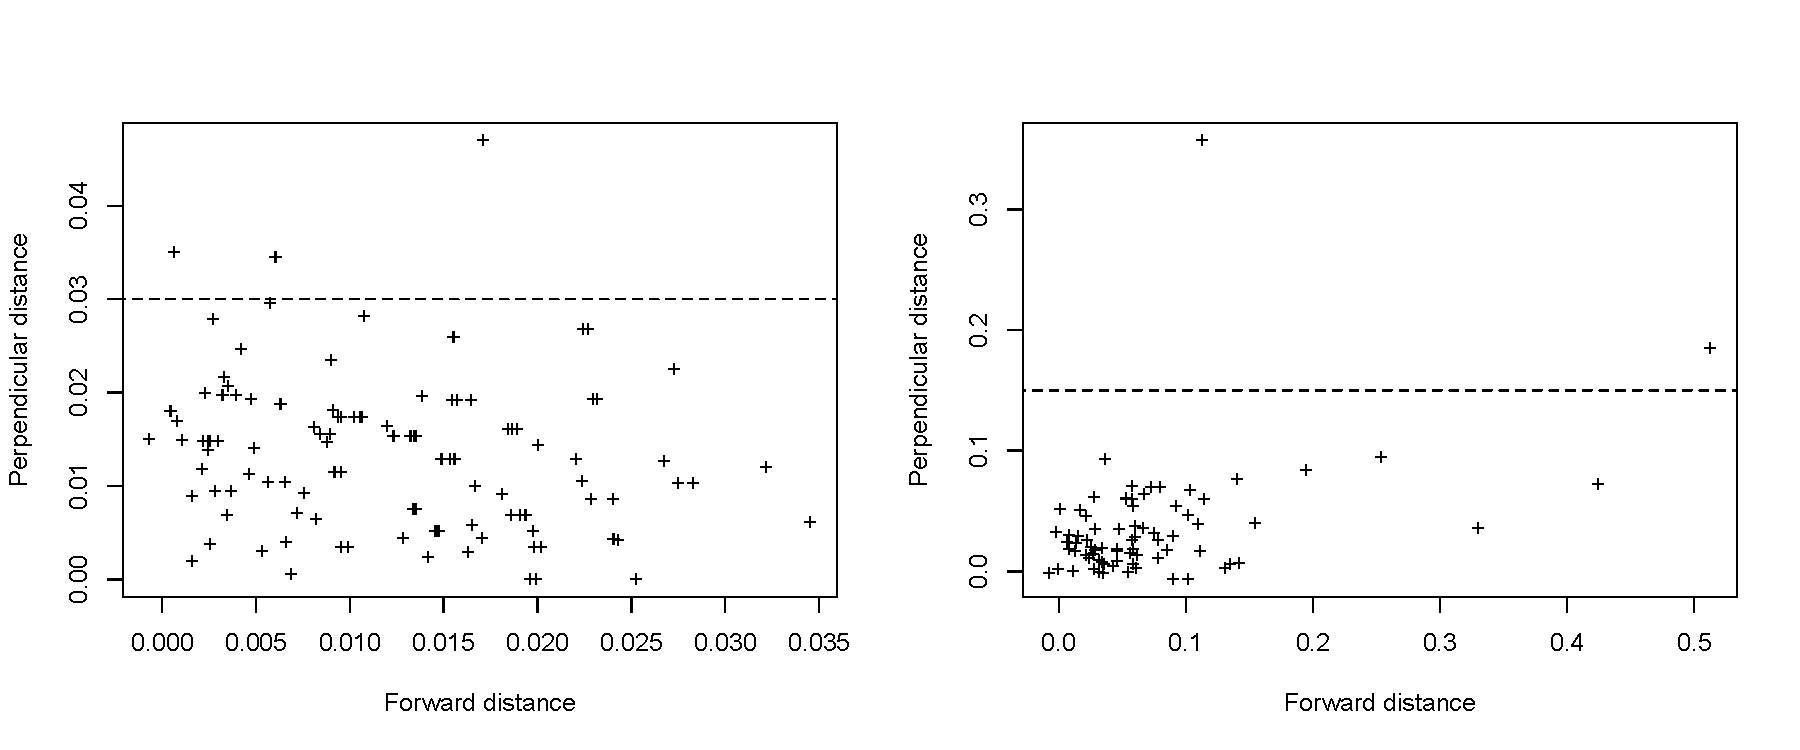
\includegraphics[scale=1]{Scatterplots.pdf}
\end{figure}

The first dataset comprises 127 detections of primates from a visual survey conducted by three sets of trained observers walking previously cut line transects in primary tropical rainforest at an elevation of 200-600m above sea level. The primates are believed to avoid the surveyors by moving some distance away from the paths, and the distribution of perpendicular distances of detected animals displays a mode at around 30m from the transect line (Figure~\ref{fig:primate.fits}).

\begin{figure}
\caption{Primate fits. The top row is perpendicular distance ($x$) plots, the bottom forward distance ($y$); the left column shows histograms and rug plots of observed data, with fitted PDFs (solid lines) overlaid, while the right column contains Q-Q plots. In the top left plot, the dashed line is the perpendicular distance detection function and the dotted line the animal distribution function $\pi(x;\boldsymbol{\phi})$. Circled points in the Q-Q plots show the points on which the Cramer-von Mises statistic is based. The bottom right Q-Q plot slopes down to reflect the fact that the CDF of forward distances is obtained by integrating from right to left. The solid line in the bottom left plot is $E_x[f_{t|x}(t|x;\hat{\boldsymbol{\beta}})]$.\label{fig:primate.fits}}
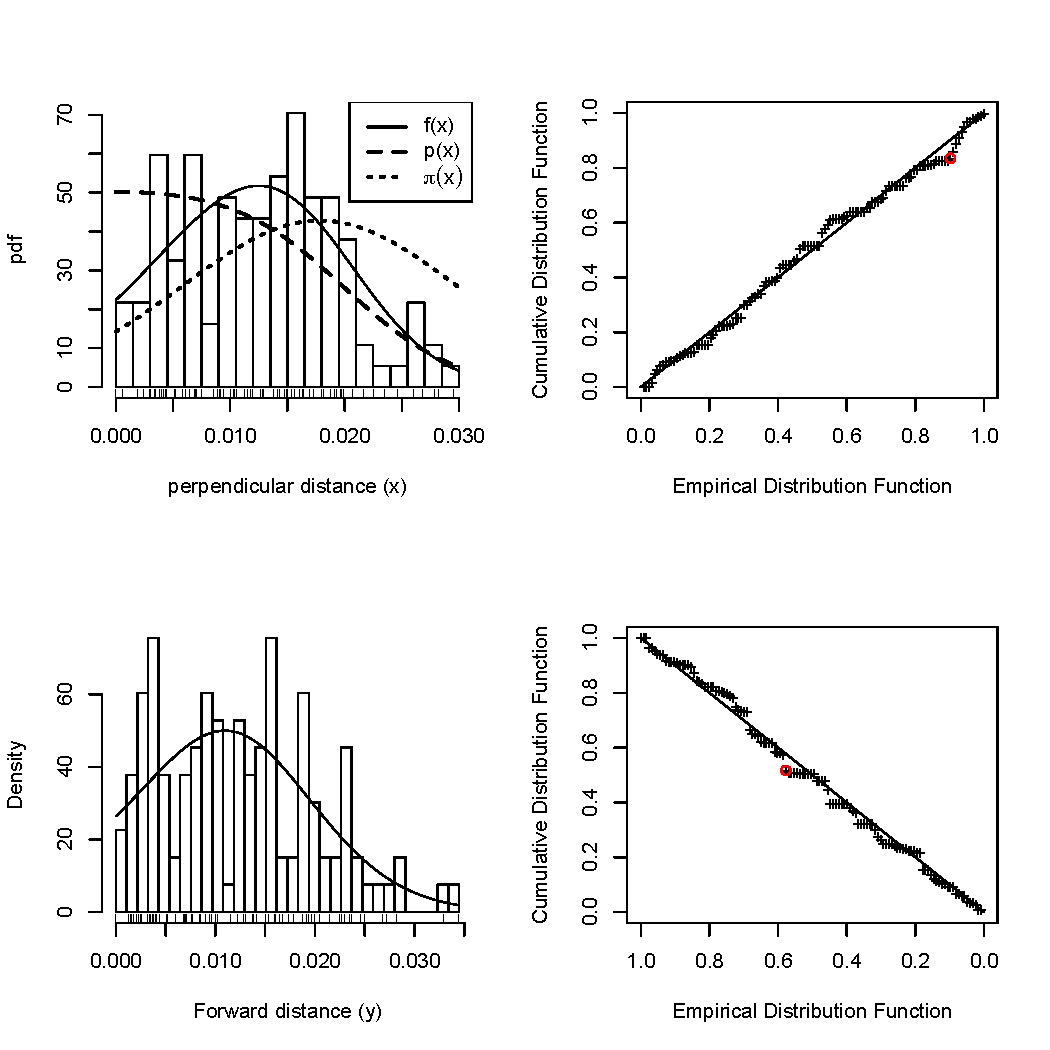
\includegraphics[scale=0.6]{PrimateFits.pdf}
\end{figure}

The second dataset comprises 76 detections  of dolphin groups by one set of observers (the ``primary platform'') on a shipboard visual survey. This survey used two independent observers and data from both observers were analysed using mark-recapture distance sampling (MRDS) methods \cite[see][for an overview of these methods]{Burt+al:15} by \cite{Canadas+al:04}. They concluded that there was substantial attraction of schools towards the transect line; the perpendicular distance data have a mode at, or very close to distance zero (Figures~\ref{fig:dolphin.fits}).

\begin{figure}
\caption{Dolphin fits.  The top row is perpendicular distance ($x$) plots, the bottom forward distance ($y$); the left column shows histograms and rug plots of observed data, with fitted PDFs (solid lines) overlaid, while the right column contains Q-Q plots. In the top left plot, the dashed line is the perpendicular distance detection function and the dotted line the animal distribution function $\pi(x;\boldsymbol{\phi})$. Circled points in the Q-Q plots show the points on which the Cramer-von Mises statistic is based. The bottom right Q-Q plot slopes down to reflect the fact that the CDF of forward distances is obtained by integrating from right to left. The solid line in the bottom left plot is $E_x[f_{t|x}(t|x;\hat{\boldsymbol{\beta}})]$.\label{fig:dolphin.fits}}
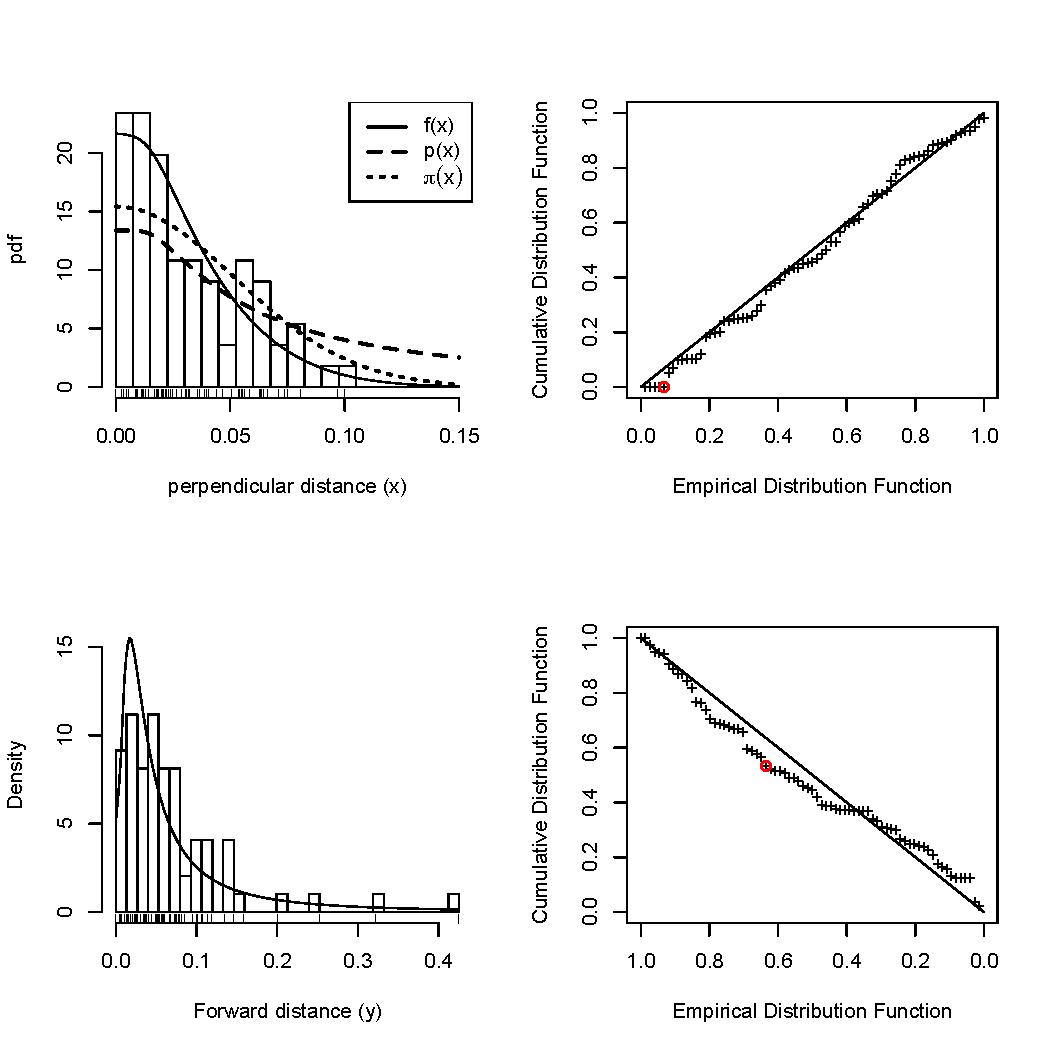
\includegraphics[scale=0.6]{DolphinFits.pdf}
\end{figure}

For each of these two surveys, we estimate ESHW in two ways: by maximising Equation~(\ref{eq:cond.lik}) and by maximising the CDS likelihood, which is obtained by dropping $f_{t|x}(\boldmath{t}|\boldmath{x})$ from Equation~(\ref{eq:cond.lik}) and setting $D_x(x;{\bmt{\phi}})=C$ to reflect the CDS assumption that objects are distributed uniformly in the vicinity of transect lines. CDS estimates were obtained using the \texttt{R} package  \texttt{Distance} \citep{Miller:15}.

\subsection{Primate survey results}

The primate data were truncated at perpendicular distance $w=0.03$ km, resulting in 4 detections being discarded. All models with $\pi_{U}$ had significantly bad fit in the $x$ dimension. Among models with non-significant goodness of fit statistics at the 5\% level, model pair $(h_{IP},\pi_{N})$ was selected on the basis of AIC, with the next best model $(h_{EP},\pi_{N})$ having an AIC larger by 8.6. However, parameters $\beta_2$ and $\beta_3$ of model $(h_{IP},\pi_{N})$ were found to be very highly correlated (estimated correlation coefficient $>0.999$) and estimates from simulations using this model did not converge properly in 40\% of cases. We therefore fitted a reduced version of $(h_{IP},\pi_{N})$, which we call $(h_{IP0},\pi_{N})$, in which the scale parameter $\beta_2$ is fixed at 1. This resulted in a model with lower AIC than $(h_{IP},\pi_{N})$ and so we base inference on model $(h_{IP0},\pi_{N})$. (The point estimates of ESHW of these two models differ by less than 0.1\%) Goodness of fit tests give p-values of 0.72 (CvM)  and 0.63 (KS) in the $x$ dimension and 0.75 (CvM)  and 0.76 (KS) in the $y$ dimension. The fits of the chosen model in perpendicular and forward distance dimensions are shown in Figure~\ref{fig:primate.fits}. The chosen model has an estimated $p(0)$ of 1.0. 

A common, if ad-hoc way of dealing with data demonstrating avoidance of the transect lines, is to fit the hazard rate model of \cite{Hayes+Buckland:83} (which is equivalent to the 2D model $h_{HB}$ in the perpendicular distance dimension). This model has a flat shoulder and although it fits poorly to these data, the rationale for using it in the presence of avoidance is that it `undoes' the avoidance to some extent by averaging through the region from which animals have fled close to the line and to which they have fled farther from the line. This fitted model is shown in Figure~\ref{fig:CDSplots}. We also fitted the model $h_{HB}$ using the forward distance data (which CDS models do not use) in addition to perpendicular distance data, with $\pi_{U}$ (which is consistent with the CDS assumption of uniform animal density). This fitted model has an AIC that is larger by 54.9 than the preferred model $(h_{IP},\pi_{N})$. 

\begin{figure}
\caption{Conventional line transect hazard rate model fits. Primate date are on the left, dolphin data on the right. \label{fig:CDSplots}}
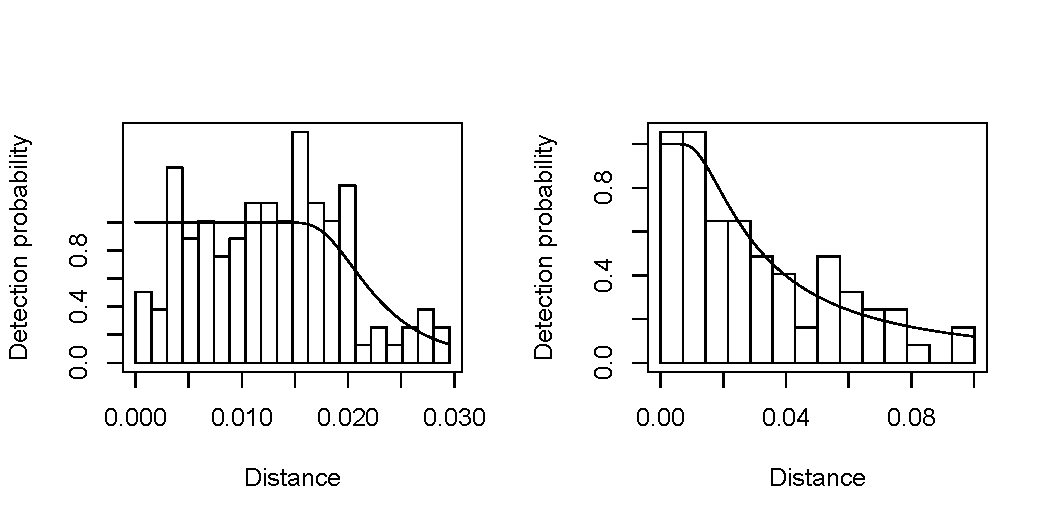
\includegraphics[scale=1]{CDSplots.pdf}
\end{figure}

The selected model $(h_{IP0},\pi_{N})$ has an estimated ESHW of 0.018 with a coefficient of variation (CV) of 12.5\% and 95\% confidence interval (CI) of (0.014, 0.023). The CDS model has an estimated ESHW that is 28\% larger at 0.023  with a CV of 5.8\%. Since estimated density is inversely proportional to ESHW (density is estimated as $\hat{D}=n/(2\times\widehat{\mbox{ESHW}}\times L)$, where $L$ is total transect length), the CDS model gives a density estimate that is some 22\% smaller than that from the selected 2D model.

The differences between the CDS estimate, which uses only perpendicular distance data and the estimates from our method, which uses 2D data (perpendicular and forward distances), are consistent with the CDS estimator not accounting adequately for the apparent avoidance of transect line by primates, and the 2D method accounting for the avoidance, albeit at the cost of additional variance due to estimating 2D hazard parameters and $\boldmath{\phi}$.

\subsection{Dolphin survey results}

The dolphin data were truncated at perpendicular distance $w=0.15$ nautical miles, resulting in two detections being discarded. Models were fitted to these data with distance distribution models $\pi_{U}$ and $\pi_{HN}$. All the models with $\pi_{U}$ had significantly bad fit. Among the models that did not have significantly bad fit, model $(h_{HB},\pi_{HN})$ was selected on the basis of AIC. All models that allow $p(0)<1$ had substantially worse AICs than model $(h_{HB},\pi_{HN})$. Goodness of fit tests give p-values for the selected model of 0.79  (CvM)  and 0.89 (KS) in the $x$ dimension and 0.24 (CvM)  and 0.42 (KS) in the $y$ dimension. The fits of the chosen model in perpendicular and forward distance dimensions is shown in Figure~\ref{fig:primate.fits}.

CDS methods were used to fit half-normal and hazard rate detection function models and the hazard rate model chosen by AIC. This fitted model is shown in Figure~\ref{fig:CDSplots}.

Model $(h_{HB},\pi_{N})$ has an estimated ESHW of 0.107 with a CV of 8.9\% and 95\% CI of (0.089, 0.127). The CDS model has an estimated ESHW some 40\% smaller at 0.064 with a CV of 18.8\%, generating a density estimate that is 67\% larger than that from model $(h_{HB},\pi_{N})$.

\cite{Canadas+al:04} obtained a density estimate of 0.123 schools per square nautical mile using MRDS methods that assume no unmodelled heterogeneity (no variables affecting detection probability of the two sets of observers that are not accounted for in the model). This will be a negatively biased estimate of density if there is unmodelled heterogeneity \citep[see][for a summary of this and related issues]{Burt+al:15}, and it is frequently the case that there is unmodelled heterogeneity on MRDS surveys. While there are ``point independence'' MRDS methods that relax the assumption of no unmodelled heterogeneity, these require uniform distribution of perpendicular distances of animals from the transect line and produce biased estimates in the presence of responsive movement. \cite{Canadas+al:04} also fitted a CDS model to the data and this produced an estimate of density 5.9 times larger than that from the MRDS method. The CDS estimate is positively biased in the presence of attraction to the transect line. Believing there to be attraction to the line, \cite{Canadas+al:04} chose what they believed to be the lesser of two evils and assumed no unmodelled heterogeneity (and hence a somewhat negatively biased estimate of density if unmodelled heterogeneity exists).

The estimated density from our method is 0.21 -- almost double the MRDS estimate and less than a third as big as the CDS estimate of \cite{Canadas+al:04}. This is consistent with the MRDS estimate being negatively biased (as is likely, due to unmodelled heterogeneity) and the CDS estimate being positively biased due to responsive movement. We do not claim that our estimator from model $(h_{HB},\pi_{HN})$ is unbiased in this case, because it seems quite likely that $p(0)$ is less than 1 \citep[][estimated it to be 0.79]{Canadas+al:04} due to animals being underwater some of the time. Although model $h_{HB}$ requires that $p(0)=1$, there are detections very close to $(x=0,y=0)$, as is evident from Figures~\ref{fig:Scatterplots} and \ref{fig:fy_x0fits}, and detections at $(x=0,y=0)$ are consistent with $p(0)<1$. However, sample size is small and this may give inadequate power to detect $p(0)<1$. In addition, the 2D method developed here assumes that $x$ does not change while animals are in view before they are detected, and this assumption may be violated for these data (although it is unclear how much this would bias estimates)

\begin{figure}
\caption{The mean estimated forward distance pdf (curve) and observed forward distance distribution (histogram) for the primate (left) and dolphin (right) detections that comprise the closest 10\% of detections to the transect line (no farther from the transect line than the dotted line shown in Figure~\ref{fig:Scatterplots}). If $p(0)$ is less than 1, the pdf has an intercept greater than zero. \label{fig:fy_x0fits}}
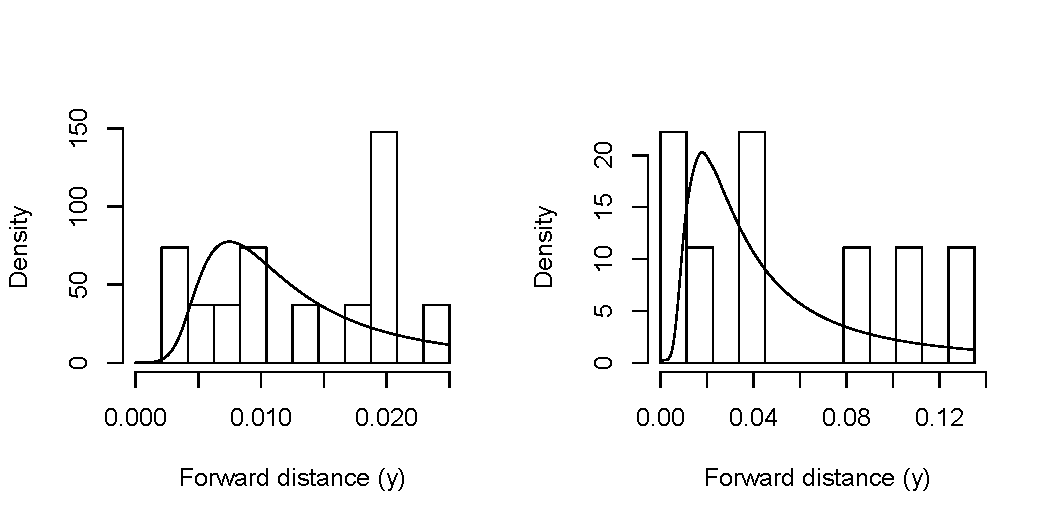
\includegraphics[scale=1]{fy_x0fits.pdf}
\end{figure}

Nevertheless, as with the primate data analysis, the difference between the CDS estimate and the 2D method estimate is consistent with the 2D method being able to account for nonuniform distribution in the perpendicular distance dimension (attraction to the transect line in this case) and the CDS estimator not being able to do so.

We investigate by simulation below, the performance of the 2D method in the presence of unknown non-uniform animal distribution, and compare its performance to CDS estimators.


\section{Simulation study}

We consider two simulation scenarios: S1 treats the 2D model fitted to the primate data as truth, S2 treats the 2D model fitted to the dolphin data as truth with simulated data drawn from  $(h_{IP0},\pi_{N})$ in S1 and $(h_{HB},\pi_{HN})$ in S2. For all simulation scenarios we estimate ESHW using our 2D method and using a CDS estimator. We measure performance in terms of estimated ESHW relative bias and 95\% CI coverage probabilities. For each scenario we simulate 1,000 surveys, with each survey having a simulated sample size equal to that of the data sets, i.e. for simulation scenario S1 $n$ = 127, and simulation scenario S2 $n$ = 76. 

The 2D model estimator of ESHW is very nearly unbiased and for S1 and unbiased for S2.  In both scenarios the 95\% confidence interval estimates have coverage close to their nominal level, while the CDS estimator has both substantial bias and very poor coverage probabilities (Table~\ref{tab:simResults}). 

\begin{table}[ht]
%\centering
\caption{Simulation results for 2D and conventional distance sampling (CDS) estimation of effective strip half width (ESHW), for simulations S1 (primates; avoidance) and S2 (dolphins; attraction). Coverage probability is the proportion of 95\% confidence interval estimates that contained the true ESHW.} \label{tab:simResults}
\begin{tabular}{ccc}
  \hline
Simulation & mean percentage  & Coverage \\ 
Scenario  & relative bias & probability \\
  \hline
S1 2D  &  -2\% & 0.95 \\ 
S1 CDS &  37\% & 0.00 \\ 
S2 2D  &   0\% & 0.94 \\ 
S2 CDS & -39\% & 0.33 \\ 
   \hline
\end{tabular}
\end{table}



\section{Discussion and Conclusions}

We have shown that when animals are not distributed uniformly with respect to distance from the line on line transect surveys, unbiased estimates of ESHW can be obtained from2D estimators that use forward distance or time to detection data as well as perpendicular distance, and that in such cases CDS estimators may be unreliable. The ability of the 2D method estimators to deal with nonuniform distribution comes from using the information in forward detection distances (or times), which CDS methods neglect. 

We have not addressed the issue of how representative density within strips is of density overall when there in nonuniform animal distribution, and this is not something that can be inferred reliably from within-strip data alone. If nonuniformity is a consequence of responsive animal movement that does not involve any animals moving into or out of strips, then density within strips is representative of density outside strips. Nonuniform density can also arise from nonrandom placement of transects, even in the presence of no responsive movement to observers. (The CDS assumption of uniformity is usually justified on the basis of random transect placement.) In some cases it may be reasonable to use estimated density at the outer edge of strips as representative of density outside strips, but in general, drawing inferences about density outside strips from estimates of density in strips may be unreliable in the presence of nonuniform distribution within strips. \cite{Marques+al:10a} discuss these issues further.

We have also shown that use of forward detection distance data and 2D inference methods provides some information on whether the key CDS assumption that $p(0)=1$ has been violated. If $f_{t|x}(t=T|x=0;\hat{\boldsymbol{\beta}})=0$, this indicates that no objects ``survive'' detection at $x=0$, i.e. that $p(0)=1$ (see Figure~\ref{fig:fy_x0fits} for example). Conversely, if $f_{t|x}(t=T|x=0;\hat{\boldsymbol{\beta}})$ is greater than zero, some animals avoid detection altogether and $p(0)<1$. In principle $p(0)$ can be estimated by $1-S(t=0,x;\hat{\boldsymbol{\beta}})$, where $\hat{\boldsymbol{\beta}}$ is the MLE of $\boldsymbol{\beta}$, but this should be done with care as small sample size may compromise the reliability of $p(0)$ estimation. The dolphin data are a case in point: it is likely from knowledge of the species and detection process, as well as from the analysis of \cite{Canadas+al:04}, that $p(0)<1$, and the histogram in Figures~\ref{fig:Scatterplots} and \ref{fig:fy_x0fits} show detections very close to zero forward and perpendicular distance, but the best model is one with $p(0)=1$. We consider the 2D method to be reliable when $p(0)$ is equal to, or close to 1. Recalling that the 2D line transect estimator can be seen as kind of removal method estimator, and that removal methods do not work well unless a large fraction of the population is removed, we believe these methods should be used with caution if $p(0)$ may be substantially less than 1. Notwithstanding this, forward detection distance data and plots like those in Figure~\ref{fig:fy_x0fits} do provide some diagnostic of whether or not $p(0)$ is 1.

We have not investigated the 2D estimator for point transects. \cite{Marques+al:10a}, \cite{Cox+al:11} and \cite{Arranz+al:14} showed how 2D data in the form of radial distance and angle can be used to estimate density in the presence of nonuniform animal distribution. But as noted above, this requires that gradient in detection probability with distance from observer does not coincide with gradient in density. Time to detection data have the potential to deal with this scenario. However, the methods we develop in this paper assume that animals are stationary while within detectable distance and for any but very short survey times $T$ (which makes time to detection data very uninformative), this is not a reasonable assumption for point transect surveys.

The 2D estimation method developed in this paper gives conservationists, managers, and others wanting to estimate animal abundance and density from line transect surveys a new tool for situations in which there is unknown object distribution within searched strips or circles. While it requires time to detection or (for line transects) forward distance at detection, these data are often quite easy to gather and we recommend that they be gathered as a matter of course where this is possible. 

It is of course better to ensure that there is uniform animal distribution within the searched area, if this is possible, than to have to estimate this distribution. And in this case CDS estimators perform well.

Finally, we return to the question posed in the title of this paper: should distance sampling methods remain 1D or move to 2D? When all CDS assumptions hold, CDS methods have a long history of performing well and we see no reason to move to 2D models in this case - although gathering time to detection or forward distance data for diagnostic purposes is still useful even then. Having shown the utility of 2D distance sampling data for line transect surveys, when the CDS assumptions that animals are uniformly distributed in the vicinity of observers is violated, we believe that in these situations distance sampling methods should be 2D, not 1D. We also note that 2D models are required to deal with stochastic animal availability; see \citep{Schweder:90}, \cite{Schweder+al:96}, \cite{Schweder+al:97}, \cite{Schweder+al:99}, \cite{Skaug+Schweder:99}, \cite{Okamura:03}, \cite{Skaug+al:04}, \cite{Okamura+al:03}, \cite{Okamura+al:06}, \cite{Okamura+al:12}, \cite{Borchers+al:13}, \cite{Langrock+al:13} and  \cite{Borchers+Langrock:ip}.

\section*{Acknowledgements}
We are grateful to Matthew Nowak from the Sumatran Orangutan Conservation Programme (SOCP) for allowing us to use the primate survey data from the Jantho Reintroduction Station. The initial survey was developed by Matthew Nowak and Serge Wich (Liverpool John Moores University) and then undertaken by the SOCP with funding from Chester Zoo. We are also grateful to the North Atlantic Marine Mammal Commission (NAMMCO) and the Faroese Museum of Natural History for allowing us to use the dolphin survey data from NASS95. MJC was funded by Australian Research Council grant FS110200057.

%\appendix
%\section{}
%\subsection{Any appendices necessary?}

\label{lastpage}

\bibliographystyle{biom}
\bibliography{dlb}

\end{document}